\section{Description of the prototype and the experimental setup} \label{sec:description_experiment}
The FOWTC hull concept is the result of the parametrical optimization procedure reported by \citet{mas2022parametric}. Following the two objectives given in Section~\ref{sec:introduction}, the experiments were conducted in such a way that they were as close as possible to the design conditions in order to allow for the verification of the numerical methods. Two main differences are, however, present: the water depth, which had to be reduced from $600\,\text{m}$ to $233\,\text{m}$, and the limitations of the software-in-the-loop approach, outlined in Section~\ref{sec:introduction} and discussed in details in Section~\ref{sec:impact_simplifications}.

The experimental campaign was conducted at the wave basin of the Numerical Offshore Tank of the University of São Paulo (TPN-USP), a squared $14\,\text{m}\times 14\,\text{m} \times 4\,\text{m}$ (length, width, depth) tank equipped with 152 active-absorption flap-type wave generators that is shown in Figure~\ref{fig:description_experiment:tanque}.
\begin{figure}[!hbtp]
	\centering
	\includegraphics[width=0.5\columnwidth]{./figures/CH-tpn.jpg}%
	\caption{Wave basin of the Numerical Offshore Tank of the University of São Paulo.} \label{fig:description_experiment:tanque}%
\end{figure}%


\subsection{Main properties of the FOWTC}
%- Caracteristicas da FOWT, RNA, ancoragem
The FOWTC concept consists of a semi-submersible hull with a $14.1\,\text{m}$ diameter central column attached to three $17.0\,\text{m}$ diameter columns arranged as an equilateral triangle, connected by rectangular pontoons $17.0\,\text{m}$ high and $6.0\,\text{m}$ wide, which was built in a 1:70 scale for the experiments. 

During design, the RNA of the IEA 15MW turbine \citep{gaertner2020definition} and the tower of the UMaine VolturnUS-S floater~\citep{allen2020definition} were mounted on top of the central column, but their inertial and structural characteristics were not preserved during the tests. Instead, the global inertial properties of the whole FOWT were matched by using a ballast system that included a moving set of weights that could be adjusted along a fuse located on top of the tower. A picture of the model is given in Figure~\ref{fig:description_experiment:modelo}, while its main properties are listed in Table~\ref{tab:description_experiment:FOWTC_properties}.
\begin{figure}[!hbtp]
	\centering
	\includegraphics[height=10cm]{./figures/foto_modelo.png}%
	\caption{Picture of the FOWTC model.} \label{fig:description_experiment:modelo}%
\end{figure}%
%\begin{figure}[!hbtp]
%	\centering
%	\fbox{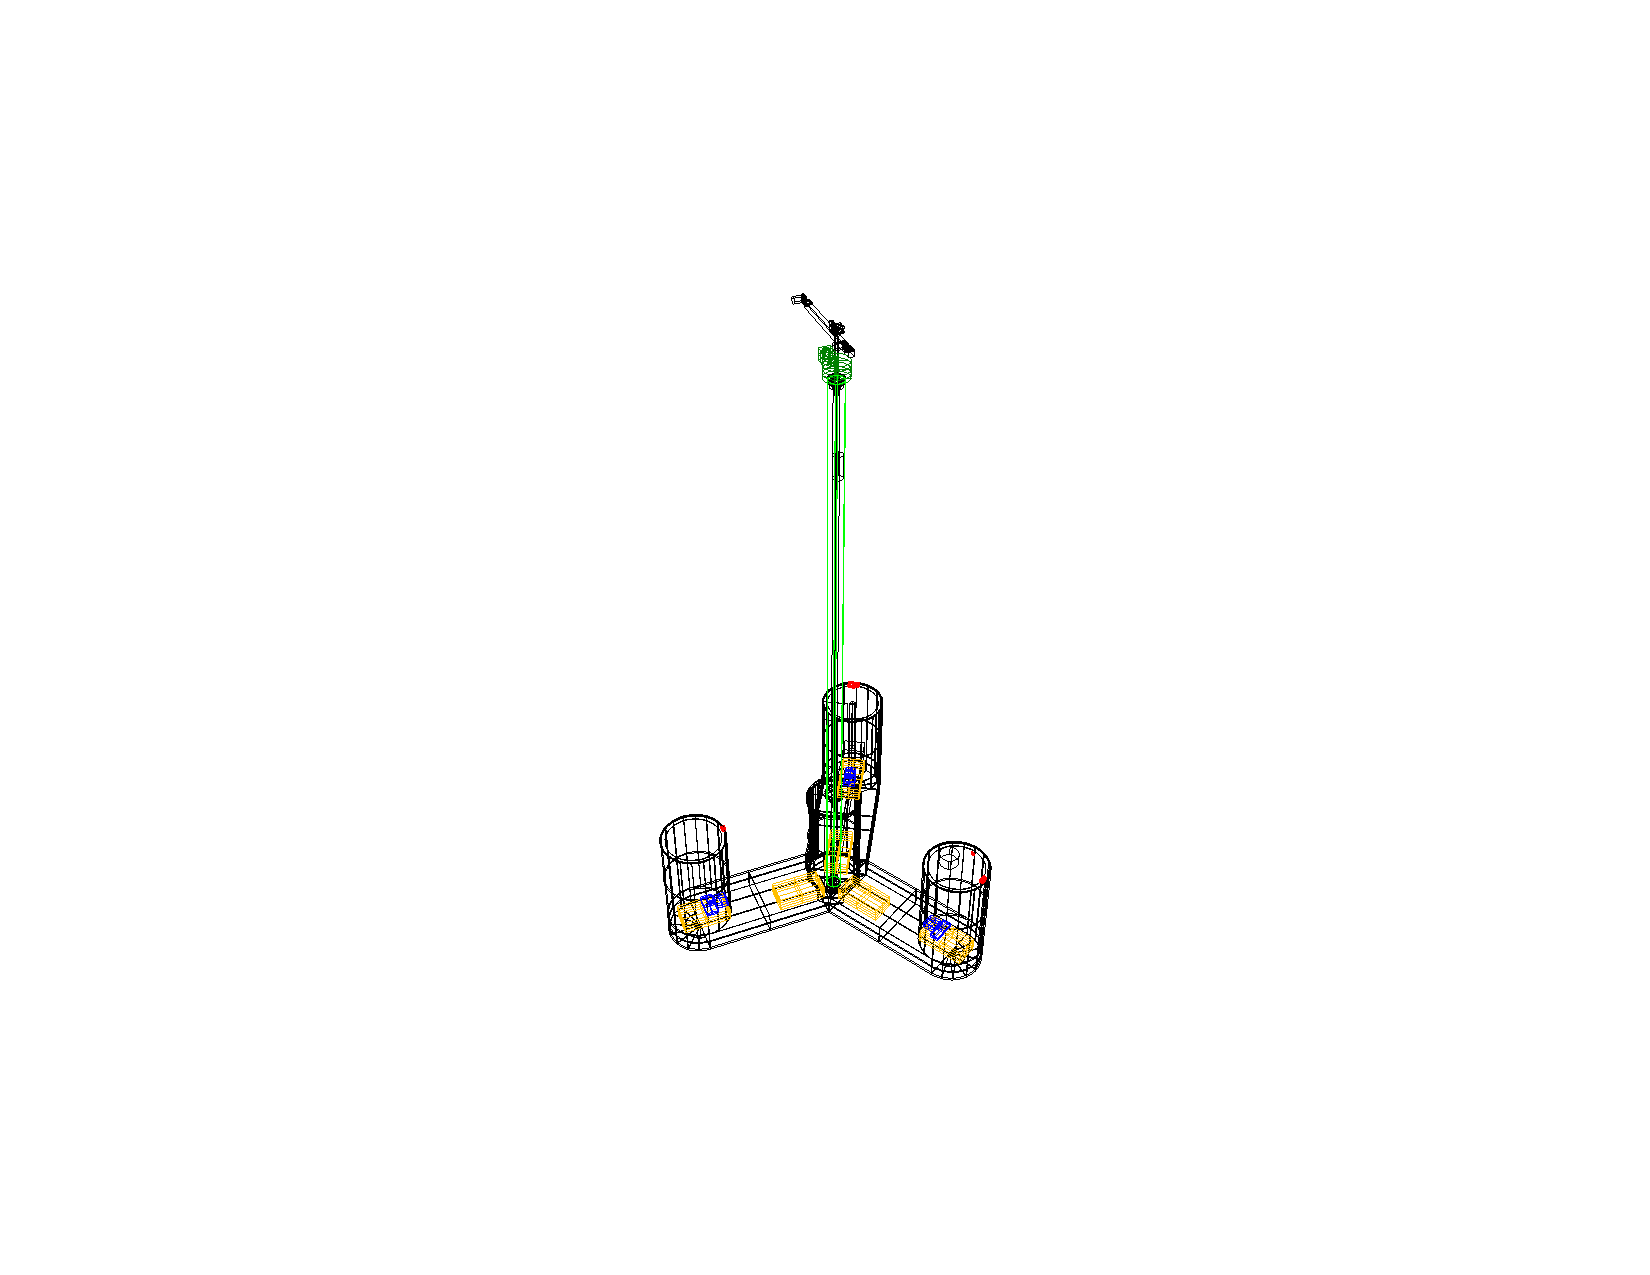
\includegraphics[trim={11cm 5cm 11cm 5cm},clip, height=10cm]{./figures/rhino_lastros.pdf}}%
%	\caption{Picture of the FOWTC model.} \label{fig:description_experiment:rhino_lastros}%
%\end{figure}%


\begin{table}[!hbtp]
	\centering
	\caption{Main properties of the FOWTC.} \label{tab:description_experiment:FOWTC_properties}   
	\begin{tabular}{lrr}
		\toprule
		& Full scale & Model Scale (1:80) \\
		\midrule
		Mass & $6 \mkern2mu 936.0 \, \text{t}$ & $13.55 \, \text{kg}$\\
		%
		Displacement & $7 \mkern2mu 351.3 \, \text{m}^3$ & $14.36 \, \text{L}$\\
		%
		Diam. of central column & $ 15.0 \, \text{m}$ & $188\,\text{mm}$ \\
		%
		Diam. of side columns & $ 9.0 \, \text{m}$ & $113\,\text{mm}$ \\			
		%
		Pitch/roll gyradius & $21.9 \, \text{m}$ & $274\,\text{mm}$ \\
		%
		Yaw gyradius & $20.3 \, \text{m}$ & $254\,\text{mm}$\\
		%
		Draft & $20.0 \, \text{m}$ & $250\,\text{mm}$ \\
		%
		KG & $15.6 \, \text{m}$ & $195 \,\text{mm}$ \\
		%
		KB & $10.0 \, \text{m}$ & $125 \,\text{mm}$  \\
		%
		BM & $8.9 \, \text{m}$ & $111 \,\text{mm}$  \\
		%
		GM & $3.3 \, \text{m}$ & $41 \,\text{mm}$  \\
        \bottomrule
        & & \\[-2pt]
		%        
        \multicolumn{3}{l}{Natural periods} \\ 
		\midrule        
		Surge/Sway & $86.3 \,\text{s}$ & $9.65 \,\text{s}$ \\
		Heave & $9.8 \,\text{s}$ & $1.09 \,\text{s}$ \\
		Pitch/Roll & $21.0 \,\text{s}$  & $2.35 \,\text{s}$\\
		Yaw & $47.0 \,\text{s}$ & $5.25 \,\text{s}$\\
		\bottomrule
	\end{tabular}%	
\end{table}%




\subsection{Software-in-the-loop approach for aerodynamic loads}
Tem que incluir o controle. Adicionar alguns resultados de teste de bancada

\subsection{Limitations of the experiment}

\subsection{Environmental conditions} \label{sec:description_experiment:envir}
- Condições de onda e vento